En esta sección se presentarán diversos artículos de investigación o tesis las cuales abordarán diversas técnicas y enfoques que se emplearon para afrontar problemas similares al de esta tesis.


\subsection{Efficient Video Classification Using Fewer Frames}
	\cite {bhardwaj2019efficient}
\subsubsection{Planteamiento del problema}
La necesidad de reducir las operaciones de punto flotante (FLOPs) y la huella de memoria. Aunque los modelos compactos actuales son más ligeros en términos de memoria, todavía requieren un número significativo de FLOPs ya que procesan todos los cuadros de un video. La propuesta de esta investigación es desarrollar modelos de clasificación de videos que procesen menos cuadros, disminuyendo así el número de FLOPs.
\subsubsection{Objetivos}

\begin{itemize}
	\item Desarrollar modelos de clasificación de video que tengan una huella de memoria pequeña (menor a 1 GB) y que sean eficientes 
	\item Crear modelos que procesen menos cuadros de video para reducir el número de FLOPs, manteniendo una alta eficiencia computacional.
	\item Utilizar un modelo maestro computacionalmente intensivo que procesa todos los cuadros para entrenar a un modelo estudiante más eficiente que procesa solo una fracción de los cuadros.
	\item Realizar una evaluación exhaustiva con tres tipos de modelos de clasificación de video: modelos recurrentes, modelos de agrupación y agregación, y modelos de agrupación y agregación eficientes en memoria.
\end{itemize}

\subsubsection{Metodología}
La metodología del documento incluye varias etapas, a partir de la recolección de datos hasta la implementación del modelo. A continuación, se presenta un resumen de la metodología:

\begin{enumerate}
	\item \textbf{Recopilación de datos}: Se utilizó el conjunto de datos YouTube-8M (versión 2017), que contiene 8 millones de videos con múltiples clases asociadas a cada video. Los videos tienen una longitud promedio de 200 segundos.
	\item \textbf{Entrenamiento del profesor y estudiante}:  Se entrena una red neuronal compleja (profesor) que procesa todos los fotogramas de un video para generar una representación detallada del mismo.Se seleccionan solo algunos fotogramas del video (cada j-ésimo fotograma) para ser procesados por la red neuronal del estudiante.e entrena una red neuronal más simple (estudiante) para que genere representaciones similares a las del profesor, utilizando solo los fotogramas seleccionados.
	\item \textbf{Minimización de pérdidas}:Se minimizan las diferencias entre las representaciones del profesor y del estudiante mediante funciones de pérdida específicas, como la pérdida de error cuadrático.
	\item \textbf{Evaluación y Comparación}:Se evalúa el rendimiento del estudiante en términos de precisión y eficiencia computacional, comparándolo con el modelo del profesor y otros métodos base.
\end{enumerate}

\begin{figure}[H]
	\centering
	\includegraphics[width=0.80\textwidth]{2/figures/Metodología_ant_1.png}
	\caption{Metodología del antecedente. Fuente:\cite {bhardwaj2019efficient}.}

	\label{1:fig}
\end{figure}


\subsubsection{Resultados}

Los resultados obtenidos se presentan en un cuadro comparativo entre los diferentes modelos utilizados en el estudio. Los modelos comparativos 1 y 2 representan otras configuraciones de modelos de aprendizaje profundo probadas por los autores para comparar la efectividad de DeepASL.
\begin{table}[h]
    \centering
    \caption{Resultados de la Clasificación de Videos Utilizando Menos Fotogramas}
    \begin{tabular}{lccccc}
        \hline
        \textbf{Modelo} & \textbf{k} & \textbf{GAP} & \textbf{mAP} & \textbf{FLOPs (Billones)} & \textbf{Tiempo de Evaluación (hrs.)} \\
        \hline
        Teacher-Skyline & N/A  & 0.811 & 0.414 & 5.058 & 13.00 \\
        Uniform-k       & 10   & 0.759 & 0.324 & 0.167 & 7.61  \\
        Uniform-k       & 20   & 0.785 & 0.363 & 0.268 & 8.20  \\
        Uniform-k       & 30   & 0.795 & 0.378 & 0.520 & 9.11  \\
        \hline
    \end{tabular}
    \label{table:video_classification}
    \begin{flushleft}
    \textit{Nota}. GAP = Precision Global Ajustada; mAP = Media de Precisión. FLOPs se refiere a las operaciones de punto flotante.
    \end{flushleft}
\end{table}



\subsection{An improved deep convolutional neural network-based YouTube video classification using textual features}
\cite{raza2024improved}
\subsubsection{Planteamiento del problema}
El artículo aborda el desafío del crecimiento exponencial del contenido de video en plataformas como YouTube, donde se suben más de 30,000 videos por hora, lo que crea la necesidad de categorizar automáticamente este contenido para hacerlo accesible a los usuarios. Las técnicas actuales de clasificación de videos, que se basan en el análisis de texto (como títulos, descripciones y etiquetas), son limitadas en precisión y no han sido suficientemente estudiadas para manejar la vasta cantidad de categorías disponibles. Además, el procesamiento de video e imagen es computacionalmente costoso, lo que impulsa el interés en enfoques basados en texto, que son más eficientes pero subdesarrollados. El artículo sugiere que se requiere un enfoque avanzado de inteligencia artificial que pueda mejorar la categorización de videos utilizando información textual de manera más eficaz y precisa.
\subsubsection{Objetivos}
\begin{itemize}
	\item Realizar un análisis exploratorio de datos de YouTube para obtener información sobre los videos y sus categorías, identificando patrones y tendencias clave.
	\item Desarrollar un modelo mejorado de red neuronal convolucional profunda (DCNN) que permita categorizar videos de YouTube con alta precisión y eficiencia.
	\item Comparar el rendimiento del modelo DCNN con otros enfoques de aprendizaje profundo, como redes neuronales recurrentes (RNN) y unidades de memoria a largo plazo (GRU), así como con modelos de aprendizaje automático tradicionales, como la regresión logística, máquinas de soporte vectorial (SVM), árboles de decisión y bosques aleatorios.
\end{itemize}

\subsubsection {Fundamento Teórico}
Dado que el procesamiento de imágenes y videos es computacionalmente costoso, el estudio explora el uso de características textuales (títulos, descripciones y etiquetas) para clasificar los videos de manera más eficiente. En este contexto, se propone un modelo de red neuronal convolucional profunda (DCNN) como enfoque principal para la categorización de videos, destacando su capacidad para manejar grandes volúmenes de datos con alta precisión. El estudio compara el desempeño del modelo DCNN con otros modelos de aprendizaje profundo, como las redes neuronales recurrentes (RNN) y las unidades de memoria a largo plazo (GRU), demostrando que el DCNN supera a estos enfoques en términos de precisión y eficiencia en la clasificación de videos.
\subsubsection {Metodología: }
	\begin{enumerate}
		\item \textbf{Adquisición de datos}: 
		\begin{itemize}
			\item Este conjunto de datos contiene 20,000 videos categorizados en 9 temas como aventura, arte y música, ciencia, deportes, entre otros.
		\end{itemize}
		
		\item \textbf{Preprocesamiento textual}:
		\begin{itemize}
			\item Limpieza de ruido en los textos de los títulos y descripciones de los videos. Se transforman los textos a minúsculas, se eliminan números, puntuaciones y espacios en blanco adicionales. El proceso incluye tokenización, eliminación de tokens no alfabéticos y palabras vacías, finalizando con la lematización para convertir las palabras a sus formas raíz.
			\item Análisis estadístico tanto a nivel observacional como de corpus. Se evalúan medidas como el tamaño promedio del vocabulario y la riqueza léxica de las descripciones.
			\item  El conjunto de datos se divide en un 80\% para entrenamiento y un 20\% para pruebas, con el objetivo de entrenar
		\end{itemize}
		
		\item \textbf{Entrenamiento del modelo}:
		\begin{itemize}
			\item Se implementan redes neuronales recurrentes (RNN) y unidades de memoria controlada (GRU) para procesar secuencias textuales. Se explica cómo estas redes manejan datos secuenciales mediante conexiones entre capas y se optimizan a través de capas de dropout y activación.
		\end{itemize}
		
		\item \textbf{Categorización de los videos}:
		\begin{itemize}
			\item Se desarrolla una red neuronal convolucional profunda (DCNN) para la clasificación de videos. El modelo utiliza capas de convolución, agrupamiento y capas densas, optimizando sus parámetros y estructura para obtener un alto rendimiento en la categorización.
		\end{itemize}
	\end{enumerate}
	\begin{figure}[H]
		\centering
		\includegraphics[width=0.5\textwidth]{2/figures/Metodología.png}
		\caption{Metodología de investigación. Fuente:\cite {raza2024improved}.}
		\label{fig:etiqueta_de_la_figura}
	\end{figure}

	\subsubsection{Resultados: }
	Los resultados del artículo se presentan en la siguiente tabla:
	
	\begin{table}[h]
		\centering
		\caption{Resultados experimentales de los modelos}
		\begin{tabular}{lccc}
			\hline
			\textbf{Modelo} & \textbf{Precisión (\%)} & \textbf{AUC (\%)} & \textbf{Puntuación F1} \\
			\hline
			DCNN & 96 & 99 & 0.95 \\
			RNN  & 92 & 97 & 0.91 \\
			GRU  & 94 & 98 & 0.93 \\
			\hline
		\end{tabular}
		\label{table:model_results}
	\end{table}







\subsection{TV News Database Indexing System with Video Structure Analysis, Representative Images Extractions and OCR for News Titles}
\cite{rozsa2022tv}

\subsubsection{Planteamiento del Problema}
El problema abordado en este trabajo es la falta de sistemas eficientes para la indexación y recuperación de contenido en archivos de video, particularmente en los programas de noticias televisivas. Muchas cadenas de televisión acumulan grandes cantidades de material de video, tanto en formatos analógicos como digitales, que no están organizados en sistemas de gestión de contenido que permitan búsquedas rápidas y reutilización del material. Esto dificulta la recuperación eficiente de información para la creación de nuevos contenidos o la supervisión del cumplimiento de las transmisiones.
\subsubsection{Objetivos}
\begin{itemize}
	\item Desarrollar un sistema semiautomático para analizar la estructura temporal de los programas de noticias televisivas.
	\item Implementar métodos de segmentación de video y extracción de imágenes representativas para mejorar la indexación de contenido.
	\item Aplicar reconocimiento óptico de caracteres (OCR) para extraer títulos de noticias y facilitar su búsqueda y recuperación.
	\item Probar el sistema propuesto en diferentes programas de noticias y evaluar su eficiencia en comparación con otros métodos.
\end{itemize}
\subsubsection{Fundamento Teórico}

El trabajo se basa en la necesidad de sistemas de gestión de contenido multimedia que puedan indexar y categorizar de manera eficiente los programas de televisión, especialmente las noticias. Se hace uso de tecnologías como la segmentación de video, la extracción de fotogramas clave y el OCR, que permite reconocer texto en imágenes. La segmentación del video se realiza analizando secuencias de fotogramas y detectando cambios significativos mediante histogramas de color y nivel de gris. Posteriormente, se extraen imágenes representativas para facilitar la navegación y búsqueda dentro de los archivos. La integración del OCR permite reconocer los títulos de las noticias, lo que facilita su búsqueda en la base de datos.

\subsubsection {Metodología }
\begin{enumerate}
	\item \textbf{Segmentación de video}:
	\begin{itemize}
		\item Se identifican puntos de inicio y fin de las tomas y se extraen imágenes representativas para cada toma. Para ello, se calcula la diferencia entre los histogramas de color de fotogramas sucesivos, utilizando métricas como la distancia de Bhattacharyya.
	\end{itemize}
	
	\item \textbf{Extracción de imágenes representativas}:
	\begin{itemize}
		\item se seleccionan imágenes representativas para cada toma con el fin de facilitar la búsqueda. Este proceso se realiza adaptando los umbrales de discriminación dependiendo de la complejidad del material.
	\end{itemize}
	
	\item \textbf{Reconocimiento óptico de caracteres (OCR)}:
	\begin{itemize}
		\item Se extrae títulos de noticias a partir de áreas predefinidas en la imagen. Se aplica preprocesamiento a las imágenes (conversión a escala de grises, umbralización) para mejorar la precisión de la extracción de texto.
	\end{itemize}
	
	\item \textbf{Evaluación del sistema}:
	\begin{itemize}
		\item  El sistema fue probado en programas de noticias de varias cadenas de televisión de Rumania, midiendo el tiempo de análisis y el número de imágenes útiles extraídas para la indexación en la base de datos.
	\end{itemize}
\end{enumerate}
\begin{figure}[H]
	\centering
	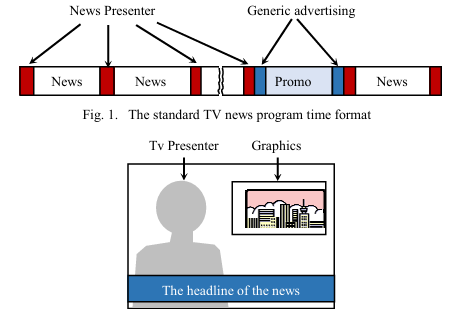
\includegraphics[width=0.5\textwidth]{2/figures/Metodologia_ant_3.png}
	\caption{Segmentación del video. Fuente:\cite {rozsa2022tv}.}
	\label{fig:etiqueta_de_la_figura}
\end{figure}

	
\subsubsection{Resultados: }

\begin{table}[h]
    \centering
    \caption{Resultados experimentales de la segmentación de video en noticias televisivas}
    \begin{tabular}{lcc}
        \hline
        \textbf{Canal de TV} & \textbf{Duración del programa (min)} & \textbf{Imágenes extraídas} \\
        \hline
        ProTV, TVR1, Kanal D, Prima TV, Intermedia & 40--45 & 800--900 \\
        \hline
    \end{tabular}
    \label{tab:segmentacion}
    \begin{flushleft}
    \textit{Nota}. Los resultados muestran la duración promedio de los programas de noticias y el número de imágenes extraídas por programa en varios canales de televisión.
    \end{flushleft}
\end{table}


\noindent \textbf{Descripción de los resultados:} Los experimentos se realizaron con programas de noticias de 40 a 45 minutos de duración de cinco canales de televisión distintos. El sistema propuesto para la segmentación de video extrajo entre 800 y 900 imágenes representativas por programa, que son utilizadas para la indexación en una base de datos de noticias televisivas. La cantidad de imágenes extraídas varía según el contenido y el estilo de producción de cada canal, pero en todos los casos se logró una segmentación precisa del contenido, facilitando la búsqueda y recuperación de material archivado.


\subsection{Shear Detection and Key Frame Extraction of Sports Video Based on Machine Learning}
\cite{wang2023shear}
\subsubsection{Planteamiento del Problema}

El trabajo aborda el problema del crecimiento exponencial de los datos de video, lo que ha generado la necesidad de herramientas eficientes para procesar, analizar y recuperar el contenido. En particular, los videos deportivos presentan desafíos debido a la diversidad de tomas y cambios rápidos en los ángulos de cámara, lo que dificulta la detección de cortes y la extracción de fotogramas clave que representen de manera precisa el contenido de las escenas.

\subsubsection{Objetivos}
\begin{itemize}
	\item Proponer un método basado en el análisis del movimiento para detectar los cortes de escena en videos deportivos.
	\item Desarrollar un algoritmo que permita la extracción automática de fotogramas clave representativos de las escenas deportivas.
	\item Reducir el volumen de datos en los índices de video mediante la selección de fotogramas clave sin comprometer la representación visual.
	\item Crear una plataforma de navegación de videos basada en fotogramas clave que facilite la búsqueda y recuperación del contenido deportivo.
\end{itemize}

\subsubsection{Fundamento Teórico}
El trabajo se fundamenta en la teoría del aprendizaje automático (ML) y el procesamiento de video, con énfasis en la eficiencia computacional. El análisis de video basado en el contenido (Content-Based Video Analysis) permite una mejor comprensión de los datos visuales mediante técnicas de visión por computadora y procesamiento de imágenes. La detección de cortes y la extracción de fotogramas clave son aspectos esenciales para la organización y recuperación de videos. Los modelos de ML, como el SVM, se utilizan para clasificar patrones en los datos visuales, mientras que los algoritmos de estimación de movimiento, basados en el bloque de coincidencia, permiten identificar transiciones entre fotogramas y escenas de manera eficiente, reduciendo el tiempo y los recursos computacionales necesarios para analizar videos extensos.

\subsubsection{Metodología}

\begin{enumerate}
	\item \textbf{Estimación del movimiento basado en bloques}:
	\begin{itemize}
		\item El algoritmo divide el video en bloques de píxeles y calcula la similitud de los bloques entre fotogramas consecutivos para identificar cambios significativos de movimiento. Esto permite detectar los cortes de escena basados en el movimiento.
	\end{itemize}
	
	\item \textbf{Detección de cortes mediante SVM}:
	\begin{itemize}
		\item El modelo de máquina de soporte vectorial (SVM) clasifica las transiciones entre fotogramas como cortes graduales o no graduales, utilizando características extraídas de los vectores de movimiento.
	\end{itemize}
	
	\item \textbf{Extracción de fotogramas clave}:
	\begin{itemize}
		\item Se utiliza un modelo de atención del usuario para determinar la relevancia de cada fotograma dentro de una escena. Los fotogramas con mayor valor de atención se seleccionan como representativos, permitiendo así una navegación más eficiente del video.
	\end{itemize}
	
	\item \textbf{Evaluación experimental}:
	\begin{itemize}
		\item El sistema fue probado en videos deportivos, midiendo su eficiencia en la detección de cortes y la capacidad de reducir el volumen de datos en los índices de video. La eficiencia se evaluó en términos del tiempo de procesamiento requerido y la precisión de la detección de transiciones graduales y no graduales. La plataforma generada permite navegar a través de los fotogramas clave para visualizar resúmenes del contenido, optimizando tanto la recuperación de la información como la experiencia de usuario.
	\end{itemize}

\end{enumerate}

\begin{figure}[H]
	\centering
	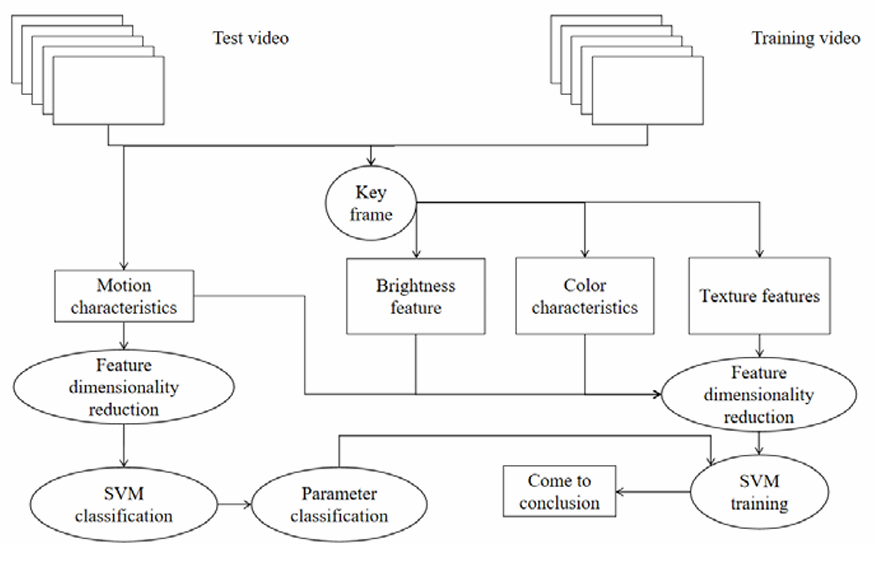
\includegraphics[width=0.5\textwidth]{2/figures/Metodologia_ant_5.png}
	\caption{Metodología del estudio. Fuente:\cite {wang2023shear}.}
	\label{fig:etiqueta_de_la_figura}
\end{figure}


\subsubsection{Resultados}

El sistema de detección de cortes y extracción de fotogramas clave propuesto demuestra ser eficiente y preciso. El uso del modelo basado en aprendizaje automático ha permitido una mejor detección de transiciones graduales y no graduales en videos deportivos, además de la extracción precisa de fotogramas clave. Este sistema puede aplicarse a múltiples tipos de videos sin necesidad de entrenamientos específicos para cada tipo, lo que mejora la eficiencia en el análisis y la recuperación de videos en entornos de alto volumen de datos.


\subsection{Research on Key Frame Extraction of Digital Image Based on Unsupervised Clustering Algorithm}
\cite{wang2023keyframe}
\subsubsection{Planteamiento del Problema}
Con el crecimiento exponencial de la información multimedia, el procesamiento eficiente de grandes volúmenes de datos de video se ha convertido en un desafío clave. Los métodos tradicionales para la extracción de fotogramas clave son ineficientes para manejar videos a gran escala y presentan limitaciones en cuanto a la precisión y velocidad de procesamiento. Esto genera una necesidad urgente de desarrollar técnicas más avanzadas que permitan extraer automáticamente los fotogramas más representativos de un video, facilitando su análisis y almacenamiento.
\subsubsection{Objetivos}
\begin{itemize}
	\item Proponer un método de extracción de fotogramas clave basado en un algoritmo de clustering no supervisado.
	\item Mejorar la precisión en la detección de fotogramas clave en videos digitales mediante el uso de algoritmos de aprendizaje automático.
	\item Reducir el tiempo de procesamiento en la extracción de fotogramas clave, optimizando la eficiencia del sistema.
	\item Validar la efectividad del algoritmo propuesto mediante simulaciones y comparaciones con modelos tradicionales de extracción de fotogramas clave.
\end{itemize}
\subsubsection{Fundamento Teórico}
El artículo se basa en el uso de algoritmos de clustering no supervisados para clasificar fotogramas de video según su similitud, permitiendo identificar aquellos más representativos de una escena. La extracción de fotogramas clave es crucial para la recuperación y análisis de contenido en videos, ya que permite generar resúmenes concisos. A diferencia de los métodos tradicionales, que dependen de intervalos de tiempo o reglas de calidad de imagen, el clustering no supervisado se enfoca en descubrir automáticamente patrones de similitud en los datos, lo que mejora la precisión de la extracción de fotogramas. La combinación con redes neuronales RBF permite modelar y ajustar mejor las trayectorias y patrones de movimiento en los videos.
\subsubsection{Metodología}

\begin{enumerate}
	\item \textbf{Extracción de características basadas en segmentación}:
	\begin{itemize}
		\item El video se segmenta en bloques de imagen, de los cuales se extraen características como el histograma de color, la textura y la forma. Estas características se agrupan en un vector para cada bloque de imagen, lo que permite realizar una comparación entre fotogramas.
	\end{itemize}
	
	\item \textbf{Cálculo de distancias de similitud}:
	\begin{itemize}
		\item Se utiliza la distancia Euclidiana para medir la similitud entre fotogramas, normalizando previamente los vectores de características. Esto permite identificar fotogramas que contienen información novedosa y los clasifica como candidatos a fotogramas clave.
	\end{itemize}
	
	\item \textbf{Algoritmo de clustering no supervisado}:
	\begin{itemize}
		\item El algoritmo realiza un análisis de movimiento y características de contenido entre los fotogramas. Agrupa fotogramas similares en clusters y selecciona aquellos que mejor representan el video. El proceso se optimiza mediante el uso de redes neuronales RBF, que ajustan las trayectorias de movimiento y optimizan la selección de fotogramas clave.
	\end{itemize}
	\item \textbf{Evaluación experimental}:
	\begin{itemize}
		\item Se realizaron simulaciones con diferentes tipos de videos para comparar el rendimiento del algoritmo propuesto con modelos tradicionales. Los resultados mostraron una mayor precisión en la extracción de fotogramas clave y una reducción en el tiempo de procesamiento.
	\end{itemize}
\end{enumerate}
\begin{figure}[H]
	\centering
	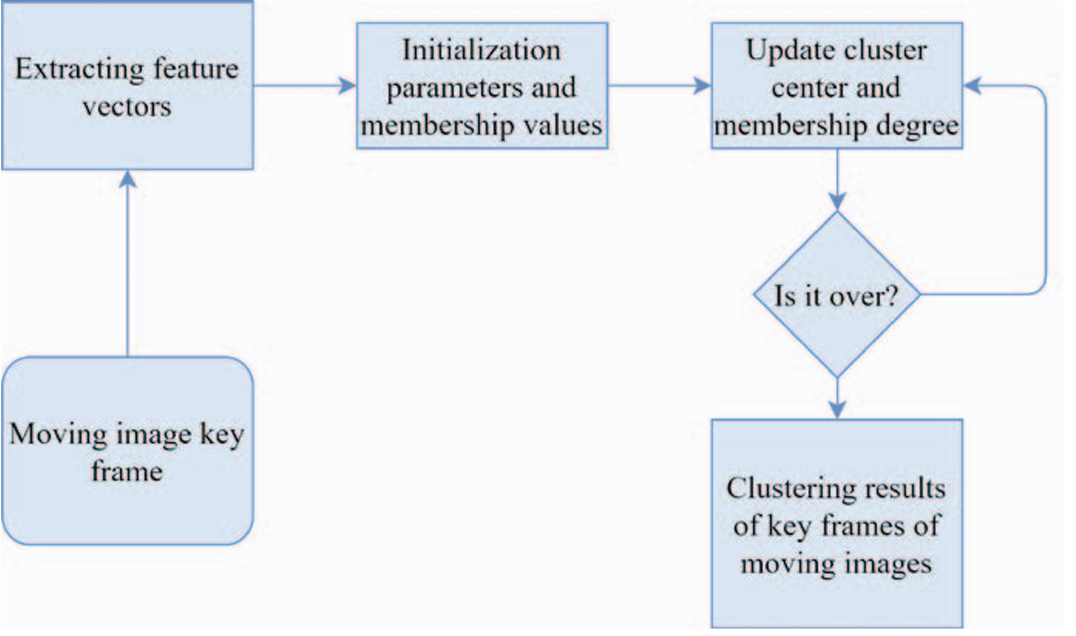
\includegraphics[width=0.5\textwidth]{2/figures/Metodologia_ant_4.png}
	\caption{Metodología del estudio. Fuente:\cite {wang2023keyframe}.}
	\label{fig:etiqueta_de_la_figura}
\end{figure}

\subsubsection{Resultados}

\begin{table}[h]
    \centering
    \caption{Resultados de la extracción de fotogramas clave y detección de cortes en videos}
    \begin{tabular}{lcc}
        \hline
        \textbf{Método} & \textbf{Precisión (\%)} & \textbf{Tiempo de procesamiento (segundos)} \\
        \hline
        Clustering no supervisado & 95.45 & 120 \\
        Modelo de mezcla gaussiana & 89.32 & 150 \\
        Algoritmo de movimiento & 92.11 & 135 \\
        \hline
    \end{tabular}
\end{table}


\noindent \textbf{Resumen de los resultados:} 
El algoritmo de clustering no supervisado propuesto demostró ser más preciso y eficiente que los métodos comparados, lo que lo convierte en una solución efectiva para la extracción de fotogramas clave en grandes volúmenes de datos de video. Esto sugiere que este enfoque tiene un gran potencial para aplicaciones en análisis de video en tiempo real y en escenarios donde se requiere procesamiento rápido de datos

\subsection{NewsVideo Summarization Combining SURF and Color Histogram Features}
\cite{liang2021news}
\subsubsection{Planteamiento del Problema}
El volumen de videos noticiosos ha crecido exponencialmente, lo que hace necesario contar con métodos eficientes para resumirlos y facilitar su consumo. Los métodos actuales de resumen de video no siempre capturan la complejidad de los videos debido a la variabilidad en las transiciones entre escenas. Además, muchos de los enfoques existentes fallan en la detección precisa de los límites entre escenas debido a los cambios en la complejidad visual, lo que resulta en resúmenes de video poco representativos.
\subsubsection{Objetivos}
\begin{itemize}
	\item Proponer un método novedoso para la detección de límites de escenas basado en características SURF.
	\item Desarrollar un algoritmo mejorado de clustering que no requiera predefinir el número de clusters y pueda adaptarse a la complejidad visual de las escenas.
	\item Reducir la redundancia en los marcos clave seleccionados para representar mejor el contenido del video noticioso.
	\item Validar la eficacia del método propuesto mediante experimentos en datasets públicos y autoconstruidos.
\end{itemize}
\subsubsection{Fundamento Teórico}
El artículo se basa en el uso de características locales, como las características SURF (Speeded Up Robust Features), que son invariantes ante rotaciones, cambios de escala y variaciones de iluminación. Estas características permiten una mayor precisión en la detección de límites entre escenas, en comparación con métodos que dependen de características globales como los histogramas de color. 

El algoritmo SURF se utiliza para identificar puntos clave en los fotogramas, lo que permite comparar la similitud entre ellos. Además, el uso de un algoritmo de clustering mejorado basado en histogramas HSV permite extraer los marcos clave más representativos de cada escena.
\subsubsection {Metodología }
\begin{enumerate}
	\item \textbf{Preprocesamiento de datos}:
	\begin{itemize}
		\item  Se eliminan elementos estáticos, como logotipos o subtítulos rodantes, que pueden interferir con la detección de límites de escena.
	\end{itemize}
	
	\item \textbf{Extraer características}:
	\begin{itemize}
		\item  Se extraen puntos de interés locales y se comparan entre fotogramas adyacentes utilizando el algoritmo FLANN para acelerar el proceso.
	\end{itemize}
	
	\item \textbf{Similitud entre fotogramas}:
	\begin{itemize}
		\item A partir de las coincidencias entre características SURF, se genera una curva de similitud que permite identificar transiciones abruptas y graduales entre escenas.
	\end{itemize}
	
	\item \textbf{Clustering basado en histogramas}:
	\begin{itemize}
		\item Se agrupan los fotogramas de cada escena según sus histogramas de color. El algoritmo ajusta dinámicamente el número de clusters para reflejar la complejidad visual de la escena.
	\end{itemize}
	
	\item \textbf{Selección de marcos clave}:
	\begin{itemize}
		\item  Se elige el fotograma más cercano al centro de cada cluster como representante clave de esa escena, garantizando que los marcos seleccionados representen fielmente el contenido del video.
	\end{itemize}
\end{enumerate}
	
\subsubsection{Resultados:}

\begin{table}[h]
    \centering
    \caption{Resultados de la detección de límites de escenas por tipo de video}
    \begin{tabular}{lcc}
        \hline
        \textbf{Tipo de Video} & \textbf{Recall (\%)} & \textbf{Precisión (\%)} \\
        \hline
        News in 30 Minutes     & 96.57 & 97.24 \\
        CCTV News              & 100.00 & 94.29 \\
        Sports Express         & 96.05 & 85.88 \\
        \hline
        \textbf{Total}         & 97.22 & 93.33 \\
        \hline
    \end{tabular}
\end{table}

\begin{table}[h]
    \centering
    \caption{Comparación de métodos de detección de límites de escenas}
    \begin{tabular}{lcc}
        \hline
        \textbf{Método} & \textbf{Recall (\%)} & \textbf{Precisión (\%)} \\
        \hline
        Ours             & 97.22 & 93.33 \\
        Feng        & 86.48 & 93.20 \\
        Wang       & 90.41 & 94.28 \\
        Rachida  & 96.49 & 95.87 \\
        TransNetV2   & 92.68 & 98.52 \\
        \hline
    \end{tabular}
    \begin{flushleft}
    \textit{Nota}. Comparación de los resultados de distintos métodos para la detección de límites de escenas.
    \end{flushleft}
\end{table}


\begin{table}[h]
    \centering
    \caption{Comparación de métodos en el dataset TVSum50}
    \begin{tabular}{lcc}
        \hline
        \textbf{Método} & \textbf{Recall (\%)} & \textbf{Precisión (\%)} \\
        \hline
        Ours             & 95.93 & 87.91 \\
        TransNetV2   & 92.56 & 92.02 \\
        \hline
    \end{tabular}
\end{table}